\chapter{Experiment Setting}
\label{cha:experiment_setting}

\textbf{ONGOING}

In this chapter, we provide a comprehensive and in-depth description of the experimental
framework designed to evaluate the performance of our LLM-driven agent.

We begin by formally defining the problem, ensuring that our study is framed
within a well-structured and precise context. We also outline the specific aspects
of the problem that our research aims to investigate, clarifying our objectives
and highlighting the novel contributions of our work.

Following this, we offer a thorough explanation of the environment used to simulate
the delivery platform. This section provides a detailed overview of the web-based
system that serves as the operational space for our agent. We describe the structure
of the platform, its key features, and how it functions as a testbed for evaluating
autonomous agents.

Finally, we discuss the selection of various Large Language Models (LLMs) used
in our experiments, including both the models that were actively tested and those
that were considered but ultimately not included in our evaluations.

\section{Problem Definition}
\label{sec:problem_definition}

As widely explained in Section \ref{sub:planning_in_llm}, the recent advancements
in Large Language Models (LLMs) have demonstrated their impressive capabilities across
a wide range of tasks. Their ability to process and reason about complex
problems opened new avenues for research, particularly in fields such as planning
and logistics. Given the power and versatility of these models, we are motivated
to further explore their potential in tackling planning and logistic challenges,
evaluating their ability to comprehend and solve such problems autonomously.

In this work, our primary focus is on assessing the inherent strengths and weaknesses
of LLMs when used in their raw form, without integrating any additional planning
frameworks, heuristic search algorithms, or explicit reasoning mechanisms on top
of them. Unlike conventional approaches that rely on dedicated pathfinding algorithms,
rule-based systems, or carefully structured reinforcement learning paradigms,
our objective is to investigate how well an LLM can independently interpret and
navigate a logistic scenario using its generative abilities alone.

One of the key aspects we wish to emphasize is that our approach remains purely
generative. In other words, rather than embedding domain-specific logic or fine-tuned
strategies within the model, we allow the LLM to operate autonomously,
generating its own understanding of the environment and devising its own
strategies for completing the given tasks. Specifically, our problem formulation
is centered around asking the LLM to provide only the \emph{next step} that moves
the agent closer to the goal, rather than generating an entire solution at once.
This step-by-step approach enables the model to iteratively refine its path based
on new observations and dynamically adapt to changing conditions. Furthermore, we
assess the reliability of each generated step by computing the uncertainty of the
model's response using the methodology detailed in Section \ref{ssub:tokens_log_probability}.

By taking this approach, we aim to answer these questions about the problem-solving
skills of LLMs in logistics problems:
\begin{itemize}
  \item To what extent can an agent, powered solely by an LLM, solve a logistic problem
    when placed in an unexpected and unfamiliar environment?

  \item What are the intrinsic limitations and strengths of this approach compared
    to traditional rule-based or algorithmic solutions?
\end{itemize}

To simulate an unexpected and dynamic environment, we designed our experiments around
a web-based platform that interacts with the agent through API calls. The
platform provides a structured yet unpredictable setting in which the agent must
operate. A critical design choice we made in our methodology was to avoid parsing
the JSON response containing the map structure. Instead, the agent receives the raw
map data (that is added to the prompt) and is expected to interpret it entirely on
its own. This decision was made to ensure that the LLM must independently derive
the necessary spatial and logistical information without relying on pre-processed
or structured inputs.

Additionally, this design choice introduces a layer of robustness: if the API
undergoes modifications, such as changes in the response format, the addition of
new parameters, or variations in data structure, the agent should still be
capable of functioning. This property aligns with our objective of evaluating the
adaptability of LLM-driven agents in dynamically changing environments, where
real-world conditions may not always remain constant.

Our experimental setup and results will be presented in detail in Chapter
\ref{cha:results_discussion}. However, to summarize our primary evaluation
criteria, we focus on testing the following goals of the LLM-based agent:

\begin{itemize}
  \item \textbf{Parcel Pickup:} We evaluate whether the agent is capable of
    successfully identifying the correct location of a parcel on the map and
    navigating to that specific tile to pick it up. This task requires the agent
    to correctly interpret spatial relationships and make movement decisions accordingly;

  \item \textbf{Parcel Delivery:} The second evaluation criterion involves
    determining whether the agent can correctly identify and reach the intended
    delivery location based on the information available in the raw map data. Since
    no explicit delivery coordinates are pre-processed for the agent, it must
    infer this information on its own.
\end{itemize}

Through these experiments, we aim to provide valuable insights into the problem-solving
capacity of LLMs in a logistic setting, evaluating their adaptability, reasoning
limitations, and potential advantages in real-world scenarios.

\section{Environment - Deliveroo.js}
\label{sec:environment_deliveroo_js}

Deliveroo.js it's an Educational Game, developed by Marco Robol for the course
on Autonomous Software Agents (ASA) by Prof. Paolo Giorgini, using the Treejs\footnote{\url{https://threejs.org/}}
framework.

The code for the server is open and che be accessed on GitHub \footnote{\url{https://github.com/unitn-ASA/Deliveroo.js}}
as well as some example of agents (with different level of complexity)\footnote{\url{https://github.com/unitn-ASA/DeliverooAgent.js}}.

The game can be played even by humans, by interacting in the browser;
technically speaking, it is a web-based platform consisting on three main components
connected to each other via sockets (implemented with Socket.io\footnote{\url{https://socket.io/}}):
\begin{itemize}
  \item \textbf{Game server}: it contains the entire logic of the game and it includes
    the implementation of client connection handler, parcel spawning, current environment
    status and so on;

  \item \textbf{Agent client}: it is the custom component that we developed to interact
    with the game server. It is a JavaScript file that connects to the server, manages
    all the logic of the agent (in our case, the LLM agent) and sends the
    actions to the server;

  \item \textbf{3D web app}: it is the visual representation of the game. It is
    a web page that connects to the server and receives the status of the game
    to render it in a 3D environment. It is not necessary for the agent to work,
    but it is useful to understand what is happening in the game.
\end{itemize}

\begin{figure}[h!]
  \centering
  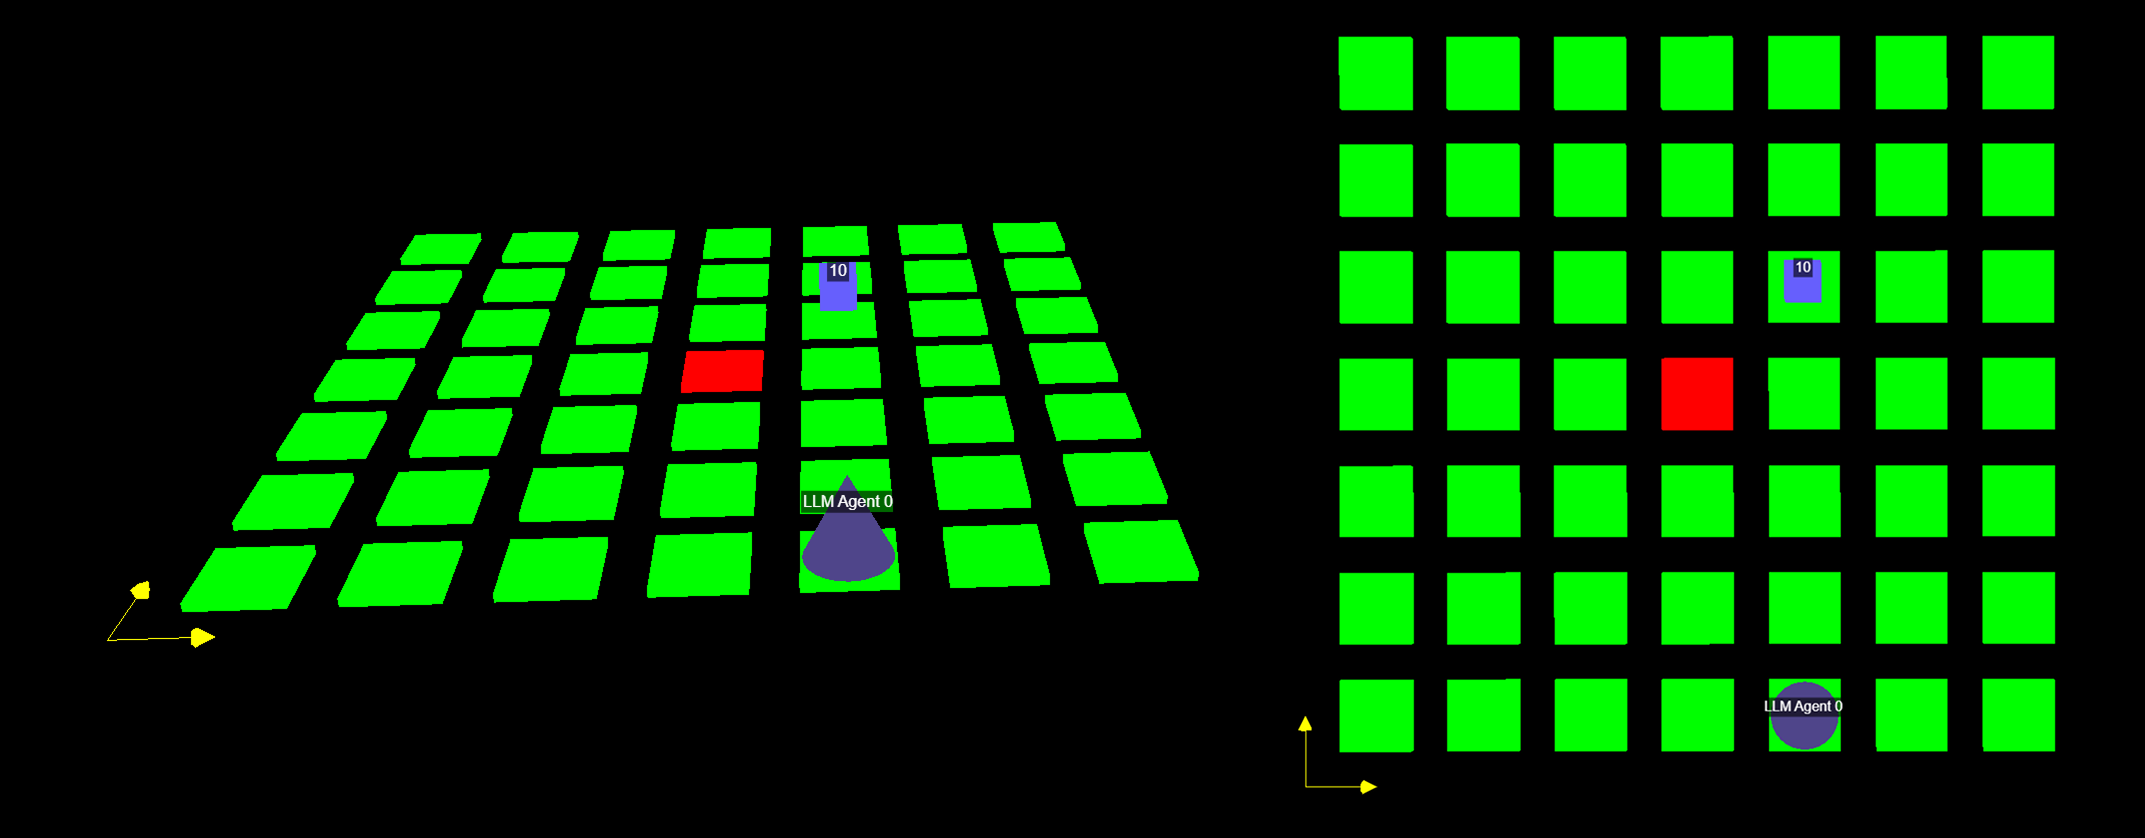
\includegraphics[width=0.65\textwidth]{images/deliveroo_js.png}
  \caption{7x7 Map in Deliveroo.js with a single central delivery zone.}
  { Source: } \label{fig:deliveroo_js}
\end{figure}

As we can see from the Figure \ref{fig:deliveroo_js}, the game is a grid of
$N \times M$ tiles where the agent can move. Right now, the $(0, 0)$ cell is in
the bottom left corner. The map is defined in a JS file (example in Listing
\ref{lst:deliveroo_map_config}) where the number inside a cell represent the type
of the cell.

\begin{lstlisting}[language=Python, caption={Example of a configuration for a 7x7 map with a single central delivery zone}, label={lst:deliveroo_map_config}]
  // 7x7 goal center deliver
module.exports = [
  [1, 1, 1, 1, 1, 1, 1],
  [1, 1, 1, 1, 1, 1, 1],
  [1, 1, 1, 1, 1, 1, 1],
  [1, 1, 1, 2, 1, 1, 1],
  [1, 1, 1, 1, 1, 1, 1],
  [1, 1, 1, 1, 1, 1, 1],
  [1, 1, 1, 1, 1, 1, 1],
];
\end{lstlisting}

There are three possible types of cells:
\begin{itemize}
  \item \textcolor{primary}{\textbf{green}} (\texttt{1}): the agent can move on
    it. They can contain multiple parcels but only one agent at a time;

  \item \textcolor{red}{\textbf{red}} (\texttt{2}): the agent can move on it and
    deliver any number of parcel it has;

  \item \textcolor{black}{\textbf{black}} (\texttt{0}): the agent can't move on
    it and they can't contain any parcel (we will not use them in our tests).
\end{itemize}

The functioning is very straight forward:

\begin{itemize}
  \item \textbf{Agents}: there can be any number of agents that can cooperate or
    compete. Each agent has a score that is increased by delivering parcels. They
    are represented as cones with their name on it on the map (`LLM Agent' in
    Figure \ref{fig:deliveroo_js} is ours).

  \item \textbf{Parcels}: they are represented as small squares with a number on
    it. The number is the reward the agent will get by delivering it. They spawn
    in random cells and they can be picked up by the agent. If they are not
    delivered in a certain amount of time, they may disappear.
\end{itemize}

\begin{lstlisting} [language=Python, caption={Example of a configuration for the server}, label={lst:deliveroo_server_config}]
  module.exports = {
  MAP_FILE: "map_file",

  PARCELS_GENERATION_INTERVAL: "5s",
  PARCELS_MAX: "1",

  MOVEMENT_STEPS: 1,
  MOVEMENT_DURATION: 50,
  AGENTS_OBSERVATION_DISTANCE: 100,
  PARCELS_OBSERVATION_DISTANCE: 100,
  AGENT_TIMEOUT: 100,

  PARCEL_REWARD_AVG: 10,
  PARCEL_REWARD_VARIANCE: "0",
  PARCEL_DECADING_INTERVAL: "infinite",

  RANDOMLY_MOVING_AGENTS: 0,
  RANDOM_AGENT_SPEED: "2s",

  CLOCK: 50,
};

\end{lstlisting}

The behavior of parcels in the system is defined through the server
configuration file. This file specifies key parameters that control parcel generation,
reward values, and decay over time. One such configuration is shown in the
example in Listing \ref{lst:deliveroo_server_config}.

Based on the server settings, a maximum number of parcels can be active simultaneously.
Each parcel is spawned at a fixed interval, with a random reward value determined
by a specified average and variance. Additionally, the configuration dictates whether
the reward remains constant or decreases over time.

In the example, parcels are generated every 5 seconds, but only one can exist at
a time. Each parcel starts with a reward value of exactly 10. Furthermore, since
\texttt{PARCEL\_DECADING\_INTERVAL} is set to \texttt{"infinite"}, the reward
does not decrease over time and the parcel will not disappear (until delivered).
This setup ensures a stable environment for testing the agent's performance.

The agent can interact with the environment using the following actions:
\begin{itemize}
  \item \textbf{up, down, left, right}: move in the specified direction, if the
    cell is empty and green or red;

  \item \textbf{pickup}: the agent can pickup a parcel in the cell it is in;

  \item \textbf{deliver}: the agent can deliver a parcel in the cell it is in:
    if it is on a delivery zone the parcel will disappear and the reward will be
    added to the player's score, otherwise it will just be dropped on the cell.
\end{itemize}

The server is responsible for transmitting events to the agent, ensuring that it
receives all relevant updates in real-time. Specifically, the following events
were utilized in our tests:

\begin{itemize}
  \item \texttt{onMap} (width, height, tiles): it sends the width and the height
    of the map, along with all the tiles in it. Tiles are currently sent as a dictionary
    \texttt{x: INT, y: INT, delivery: BOOL, spawner: BOOL} where \texttt{delivery}
    is true if the tile is a delivery zone and \texttt{spawner} is true if a
    parcel can spawn on it.

  \item \texttt{onYou} (id, name, x, y, score ): it sends the id, the name, the
    x and y coordinates and the score of the agent connected the code is
    piloting.

  \item \texttt{onParcelsSensing} async (perceived\_parcels): it is an async function
    that sends the parcels that the agent can see at any time. The parcels are
    sent as a dictionary \texttt{x: INT, y: INT, reward: INT} where \texttt{x}
    and \texttt{y} are the coordinates of the parcel and \texttt{reward} is the
    reward the agent will get by delivering it.
\end{itemize}

\section{LLM Models}
\label{sec:llm_models}

\subsection{Open Source}

\subsection{OpenAI}